\documentclass[aip,jcp,reprint,noshowkeys,superscriptaddress]{revtex4-1}
\usepackage{graphicx,dcolumn,bm,xcolor,microtype,multirow,amscd,amsmath,amssymb,amsfonts,physics,wrapfig,txfonts,siunitx}
\usepackage[version=4]{mhchem}
%\usepackage{natbib}
\bibliographystyle{achemso}

\newcommand{\ie}{\textit{i.e.}}
\newcommand{\eg}{\textit{e.g.}}
\newcommand{\alert}[1]{\textcolor{black}{#1}}
\usepackage[normalem]{ulem}
\newcommand{\fk}[1]{\textcolor{blue}{#1}}
\newcommand{\titou}[1]{\textcolor{red}{#1}}
\newcommand{\trashPFL}[1]{\textcolor{red}{\sout{#1}}}
\newcommand{\PFL}[1]{\titou{(\underline{\bf PFL}: #1)}}
\newcommand{\toto}[1]{\textcolor{green}{#1}}
\newcommand{\trashAS}[1]{\textcolor{green}{\sout{#1}}}
\newcommand{\AS}[1]{\toto{(\underline{\bf AS}: #1)}}
\newcommand{\ant}[1]{\textcolor{orange}{#1}}
\newcommand{\SupInf}{\textcolor{blue}{Supporting Information}}

\newcommand{\mc}{\multicolumn}
\newcommand{\fnm}{\footnotemark}
\newcommand{\fnt}{\footnotetext}
\newcommand{\tabc}[1]{\multicolumn{1}{c}{#1}}
\newcommand{\QP}{\textsc{quantum package}}

\newcommand{\EHF}{E_\text{HF}}
\newcommand{\EDOCI}{E_\text{DOCI}}
\newcommand{\EFCI}{E_\text{FCI}}
\newcommand{\Ndet}{N_\text{det}}
\newcommand{\Nbas}{N}

\usepackage[
	colorlinks=true,
    citecolor=blue,
    breaklinks=true
	]{hyperref}
\urlstyle{same}

\begin{document}

\newcommand{\LCPQ}{Laboratoire de Chimie et Physique Quantiques (UMR 5626), Universit\'e de Toulouse, CNRS, UPS, France}

\title{Seniority and hierarchy configuration interaction for radicals and excited states}

\author{F\'abris Kossoski}
\email{fkossoski@irsamc.ups-tlse.fr}
\affiliation{\LCPQ}
\author{Pierre-Fran\c{c}ois Loos}
\email{loos@irsamc.ups-tlse.fr}
\affiliation{\LCPQ}

% Abstract
\begin{abstract}
{\bf Abstract:} 
%\bigskip
%\begin{center}
%        \boxed{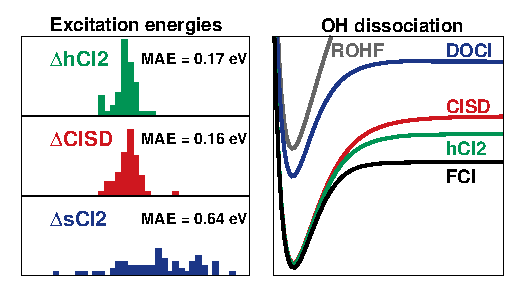
\includegraphics[keepaspectratio,width=2in]{TOC}}
%\end{center}
%\bigskip
\end{abstract}

% Title
\maketitle


%%%%%%%%%%%%%%%%%%%%%%%%%%%%%%%%%%%%%%%%%%%%%%%%%%
\section{Introduction}
\label{sec:intro}
%%%%%%%%%%%%%%%%%%%%%%%%%%%%%%%%%%%%%%%%%%%%%%%%%%


Configuration interaction (CI) offers a systematic way to solve the many-body electronic structure problem. \cite{SzaboBook,Helgakerbook}
By including progressively more determinants in the Hilbert space, the wave function becomes increasingly closer to the exact one, and so does the electronic energy.
In full CI (FCI), all determinants are accounted for and the problem is solved exactly (for a given basis set).
In practice, however, one resorts to approximate CI models, where only the determinants that satisfy a given criterion are included in the truncated Hilbert space.

The most well-known CI route is excitation-based.
Starting from a reference determinant, typically the Hartree-Fock (HF) determinant,
one generates all determinants that are connected to it by excitating at most $e$ electrons.
The excitation degree $e$ thus defines the order of the approximate CI model:
CI with single excitations (CIS); CI with single and double excitations (CISD), CI with single, double and triple excitations (CISDT), and so on.
A different CI route is based on the seniority number $s$ (the number of unpaired electrons in a given determinant).
In seniority-based CI (sCI) \cite{Bytautas_2011,Allen_1962,Smith_1965,Veillard_1967}, there is no reference determinant, and one accounts for all determinants having seniority equal or less than $s$.
For systems with an even number of electrons, the first approximate model is defined by $s=0$ (sCI0), usually refered to as doubly-occupied CI (DOCI),
which is followed by the higher-order models sCI2, sCI4, and so on.
For an odd number of electrons, the seniority route follows along odd numbers of $s$: sCI1, sCI3, and so on.
%Limited studies for radicals and excited states

%sCI works well to describe molecular dissociation \cite{Bytautas_2015,Alcoba_2014,Alcoba_2014b}
%For small systems, FCI is still attainable and one can thus gauge the performance of approximate CI models.
We have recently introduced a third CI route, hierarchy CI (hCI), \cite{Kossoski_2022}
where the Hilbert space is partitioned according to a hierarchy parameter $h$ that combines the excitation degree $e$ and the seniority number $s$ according to $h = (e+s/2)/2$.
This definition ensures that all types of determinants whose number share the same scaling with system size are included at the same hierarchy $h$.
For different properties and closed-shell molecular systems, 
hCI was found to display an overall faster convergence to the FCI results than the traditional excitation-based CI. \cite{Kossoski_2022}
However, hCI has only been defined for a closed-shell reference, thus systems with an even number of electrons.
Here, our first goal is to generalize hCI for open-shell systems and to assess the performance of this class of methods by performing calculations for various properties of several radicals.
%A generalization of the method for open-shell systems has not yet been proposed.
%excitations of increasingly higher order give rise to a systematically improvable sequence of CI methods:
The second goal is to evaluate how perturbation theory, more precisely the second-order Epstein-Nesbet (EN2) perturbative correction, \cite{Garniron_2019}
impacts different properties of ground-state closed-shell systems and radicals, for excitation-based, sCI and hCI methods.

%Whereas the first CI root represents the electronic ground state, higher-lying roots give access to excited states.
%Similarly, the favourable results of hCI when compared to excitation-based CI for ground states raises the question on how well it can describe excitation energies.
%The performance of excitation-based CI for excited states is well stablished, \cite{} but remains an open question for sCI methods,
Inspired by the results of hCI for ground-state closed-shell systems, \cite{Kossoski_2022} our third goal is to define and assess the accuracy of hCI models for excited states.
Furthermore, to the best of our knowledge, sCI models have not yet been directly used to target excited states,
despite the growing number of methods that exploit the concept of seniority number,
for both ground
\cite{Limacher_2013,Limacher_2014,Tecmer_2014,Boguslawski_2014a,Boguslawski_2015,Boguslawski_2014b,Boguslawski_2014c,Johnson_2020,Henderson_2014,Stein_2014,Henderson_2015,Chen_2015,Bytautas_2018,Marie_2021,Boguslawski_2021,Tecmer_2022,Mamache_2023} 
and excited states.
\cite{Boguslawski_2016b,Boguslawski_2016c,Boguslawski_2019,Nowak_2019,Kossoski_2021,Marie_2021,Tecmer_2022,Rishi_2023,Nowak_2023} 
Our fourth goal is therefore to introduce and gauge sCI models for excited states.
There are two possible approaches to target excited states with CI.
One can employ the ground-state HF orbitals and obtain excitation energies from the higher-lying eigenvalues of the CI matrix, which we refer to as ground-state based approach.
Instead, one may optimize the orbitals for the excited state of interest (described with an appropriate reference), followed by a separate CI calculation,
in a so-called state-specific approach ($\Delta$CI).
There has been a recent surge in the development of state-specific methods, covering 
single-reference and multiconfigurational self-consistent field,
\cite{Ziegler_1977,Burton_2021,Shea_2018,Tran_2019,Tran_2020,Hardikar_2020,Burton_2022,Hanscam_2022,Kossoski_2023,Marie_2023}
% add references for SCF
%\cite{Ziegler_1977,Burton_2021}
%multiconfigurational SCF, \cite{Shea_2018,Tran_2019,Tran_2020,Hardikar_2020,Burton_2022,Kossoski_2023,Marie_2023}
density functional theory, 
\cite{Filatov_1999,Kowalczyk_2011,Kowalczyk_2013,Gilbert_2008,Barca_2018,Hait_2020,Hait_2021,Hardikar_2020,Zhao_2020,Levi_2020,Carter-Fenk_2020,Toffoli_2022,Schmerwitz_2022}
and coupled-cluster (CC)
\cite{Piecuch_2000,Mayhall_2010,Lee_2019,Kossoski_2021,Marie_2021,Rishi_2023}
methods.
In particular, by employing a minimal configuration state function (CSF) reference, 
we have recently shown that excitation-based $\Delta$CI models deliver far more accurate excitation energies than the ground-state based analogues. \cite{Kossoski_2023}
Based on this promising set of results for excitation-based CI, here we explore both ground-state based and state-specific approaches for sCI and hCI models.




%%%%%%%%%%%%%%%%%%%%%%%%%%%%%%%%%
\section{Hierarchy configuration interaction}
\label{sec:hCI}
%%%%%%%%%%%%%%%%%%%%%%%%%%%%%%%%

%We introduced hCI for closed-shell systems, \cite{Kossoski_2022}
We introduced hCI \cite{Kossoski_2022} as a truncation of the Hilbert space based on a two-dimensional map of determinants (see Fig.~\ref{fig:hci})
built from their seniority $s$ and their excitation degree $e$ with respect to a reference determinant.
It is built such that all classes of determinants whose number $\Ndet$ share the same scaling with the number of basis functions $N$ enter at the same order of truncation,
which means moving diagonaly in this seniority-excitation map.

The first order for a closed-shell reference determinant is hCI1, which accounts for all single excitations (as CIS) 
plus all paired doubled excitations (two electrons promoted from the same occupied orbital into the same virtual orbital).
For both types of determinants, their number scales as $N^2$, and thus should be taken into account at the same hierarchy of hCI ($h=1$ in this case).
At the next integer order, hCI2 accounts for all types of determinants where $\Ndet$ scale as $N^4$ or less.
That means all single and double excitations (as CISD), plus the subset of triple excitations that leave only two unpaired electrons, 
plus the subset of quadruple excitations where no electrons are unpaired.
More generally, in hCI, the number of determinants $\Ndet$ scales polynomially with the number of basis functions $N$ as $N^{2h}$.
Similarly, for excitation-based CI, $\Ndet$ scales as $N^{2e}$, where $e$ is the excitation degree.

Here we generalize hCI for an arbitrary type of reference Slater determinant and for odd number of electrons.
With respect to a given reference determinant, we define the hierarchy $h$ of a target determinant as
\begin{equation}
  \label{eq:h}
  h = \frac{e+ (s-s_0)/2}{2},
\end{equation}
where $s$ and $s_0$ denote the seniority of target and reference determinants, respectively, and $e$ represents the excitation degree that connects the two determinants.
The term $(s-s_0)/2$ is always an integer, with $s$ and $s_0$ being even (odd) for systems with an even (odd) numbers of electrons, whereas $e$ is also an integer.
Therefore, $h$ can assume integer or half-integer values, for any type of reference determinant.
For a given hCI model defined by the hierarchy $h$, all determinants having a hierarchy less than or equal to $h$ are selected.
Notice that Eq.~\eqref{eq:h} simplifies to the previous definition \cite{Kossoski_2022} for the case of a closed-shell reference determinant, when $s_0 = 0$.

The above definition ensures that all types of determinants with a given scaling enter at the same hierarchy $h$.
% computational scaling
We show in Fig.~\ref{fig:hci} how the seniority-excitation map of determinants is partitioned for a closed-shell reference, and for open-shell references with one or two unpaired electrons.
%the different types of determinants that are accessed for a closed-shell reference, and for open-shell references with one or two unpaired electrons.
hCI can also be interpreted as the CI model that provides increasingly more dissimilar determinants from the given reference determinant.
This dissimilarity is represented by the hierarchy $h$, which accounts for differences in orbital occupation (through the excitation degree $e$)
and differences in the number of unpaired electrons (through the term $(s-s_0)/2$).
 



%%%%%%%%%%%%%%%%%%%%%%%%%%%%%%%%%
\section{Computational details}
\label{sec:compdet}
%%%%%%%%%%%%%%%%%%%%%%%%%%%%%%%%

The hCI models introduced here were implemented in {\QP} \cite{Garniron_2019} through a straightforward modification of the
\textit{configuration interaction using a perturbative selection made iteratively} (CIPSI) algorithm. \cite{Huron_1973,Giner_2013,Giner_2015,Garniron_2018}
By allowing only for the determinants that are connected with the reference determinant(s) up to a given maximum hierarchy $h$,
the CIPSI algorithm is restricted to the truncated Hilbert space defined by the reference determinant(s) and the value of $h$.
{\QP} \cite{Garniron_2019} was also employed to perform all the CI calculations presented here.
In a given calculation, the energies are considered to be converged when the (largest) renormalized EN2 correction computed in the truncated Hilbert space 
lies below \SI{0.01}{\milli\hartree}. \cite{Garniron_2018}
%by spanning the most important regions of the truncated Hilbert space
This selected CI procedure requires considerably fewer determinants than the total number of determinants in the truncated Hilbert space,
while delievering fairly converged absolute and excitation energies.
The ground- and excited-state CI energies are obtained with the Davidson iterative algorithm. \cite{Davidson_1975}
For a given approximate CI model, we futher evaluated the bare and the renormalized EN2 perturbative correction. \cite{Garniron_2019} 
This calculation involves a single loop over the determinants left outside the truncated (internal) space but connected to it via at most double excitations.
Looping over these external doubly excited determinants has a computational scaling equal to $\Ndet$,
thus $\order*{N^{2e+4}}$ for excitation-based CI and $\order*{N^{2h+4}}$ for hCI, where $e$ or $h$ define the internal CI space.
For example, hCI2 and CISD present a $\order*{N^6}$ computational scaling, whereas hCI2+EN2 and CISD+EN2 scale as $\order*{N^8}$,
though with a small prefactor stemming from the EN2 calculation.

To gauge the performance of hCI against excitation-based and seniority-based CI for radical systems,
we have calculated the ground-state potential energy curves (PECs) for the dissociation of four radical systems:
\ce{OH}, \ce{CN}, vinyl (\ce{C2H3}), and \ce{H7}.
These calculations employed the ground-state restricted open-shell HF orbitals and the frozen core approximation.
%which display a variable number of bond breaking.
The equilibrium geometry of vinyl was taken from Ref.~\onlinecite{Loos_2020},
%also reproduced in the \SupInf,
and the PECs were computed along the \ce{C=C} double bond breaking coordinate, with the remaining internal coordinates kept frozen.
For \ce{H7}, we considered equally spaced and linearly arranged hydrogen atoms, and the PECs were computed along the symmetric dissociation coordinate.
The results were analyzed along the same lines of our report on hCI for closed-shell systems. \cite{Kossoski_2022}
Namely, for the different CI models considered here, 
we evaluated the convergence of the non-parallelity error (NPE), the distance error, the harmonic vibrational frequencies, and the equilibrium bond lengths, as functions of $\Ndet$.
The NPE (distance error) of a given level of theory is defined as the maximum minus (plus) the minimum differences between its corresponding PEC and the FCI one, for a given range of coordinates.
Details about how the harmonic vibrational frequencies and equilibrium geometries were obtained from the calculated PECs,
and the ranges defining the NPE and distance errors can be found in the \SupInf.

The various CI models introduced here were further assessed based on calculated vertical excitation energies for 60 electronic states,
from 18 closed-shell systems and 8 radicals, with geometries extracted from the QUEST database. \cite{Veril_2021}
The full set of excited states and calculated excitation energies, for the various CI models, are provided in the {\SupInf}.
We employed the aug-cc-pVDZ basis set for systems having up to three non-hydrogen atoms and the 6-31+G(d) basis set for the larger ones.
Core orbitals were frozen.
For the radicals, we further impose the CI solutions to be eigenstates of the spin angular momentum operator, which implies accounting for a set of appropriate spin-flipped determinants.
In this sense, our CIS calculations for radicals actually correspond to the so-called extended CIS, \cite{Maurice_1996} and similarly for the other hCI and excitation-based CI models.
We performed calculations following both the standard ground-state based CI route and the state-specific CI route. \cite{Kossoski_2023}
For the latter, we employed the state-specific orbitals obtained in Ref.~\onlinecite{Kossoski_2023}.
Notice that, in contrast to excitation-based CI, the energies obtained with sCI and hCI models are not invariant under rotations within the occupied and virtual subspaces.
The computed excitation energies were compared against the reference values provided in the QUEST database. \cite{Veril_2021}
%For completeness, we also reproduce the geometries in the \SupInf.

The restricted HF solution (restricted open-shell HF for the open-shell systems) was taken as reference determinant for the hCI ground state calculations.
For the state-specific hCI calculations, we employed a minimal CSF reference, \cite{Kossoski_2023}
meaning a single open-shell determinant for the doublet excited states and a single CSF for the singly-excited states from closed-shells.
As for the seniority-based CI models, 
we considered sCI1 for both ground and (state-specific) excited state calculations for the open-shell systems (odd number of electrons).
For the closed-shell systems (even number of electrons), we explored two models.
In the sCI2/sCI0 model, the ground state was described with sCI0 and the excited state with sCI2, which is the minimal seniority-based CI model for computing excitation energies for closed-shells.
Further including the $s=2$ sector for the ground state calculations gives rise to the sCI2/sCI2 model.
CI models carrying the $\Delta$ symbol denote a state-specific approach, whereas those without it imply a ground-state based approach.
% comments on the different references 


%%%%%%%%%%%%%%%%%%%%%%%%%%%%%%%%
\section{Results and discussion}
\label{sec:res}
%%%%%%%%%%%%%%%%%%%%%%%%%%%%%%%%


%%%%%%%%%%%%%%%%%%%%%%%%%%%%%%%%
\subsection{hCI for radicals}
\label{sec:res_A}
%%%%%%%%%%%%%%%%%%%%%%%%%%%%%%%%

% redefine the distance errors because of negative values?
% vinyl missing point at 5.2 for s3i+pt2 and at 2.0 for s5+pt2
% CN correct dissociating part for h4 and h3.5
% H8 missing points for Q+pt2
% H8 missing 9.0 for T+pt2

The full set of PECs for the open-shell systems (\ce{OH}, \ce{CN}, \ce{H7}, and vinyl) are presented in the {\SupInf},
along with the NPEs, distance errors, equilibrium bond lengths and harmonic vibrational frequencies, plotted as a function of $\Ndet$ for the different CI models.
The present results for open-shell systems are discussed in detail in the following,
and display similar trends to the ones previously reported for closed-shell systems. \cite{Kossoski_2022}
hCI typically improves the convergence of the different properties when compared to excitation-based CI.
Concerning the NPEs, such improvement is clear for \ce{OH} and \ce{CN} (involving a single bond breaking), less so for vinyl (double bond breaking),
whereas for \ce{H7} (multiple bond breaking), hCI and excitation-based CI perform similarly.
This behavior had also been observed for dissociation of closed-shell systems. \cite{Kossoski_2022}
The same trend is observed for the distance error, although the improvement from excitation-based CI to hCI is less marked than for the NPEs.
hCI further leads to a faster convergence of the equilibrium geometry of \ce{CN}, while comparable results are found for the geometries of the other systems.
Meanwhile, a clear improvement from excitation-based CI to hCI is observed for the vibrational frequencies, except for \ce{H7}, where no difference is found.

%orbital optimization?

We further assesssed the effect of the EN2 perturbative correction for both the open-shell systems studied here 
and the closed-shell systems (\ce{HF}, \ce{F2}, \ce{N2}, ethylene, \ce{H4}, and \ce{H8}) addressed in our first report on hCI. \cite{Kossoski_2022}
The full set of PECSs is shown in the {\SupInf}.
At stretched geometries, the perturbative correction can lead to kinks and large jumps in the PECs.
Such problems were encountered at some levels of CI for \ce{CN}, vinyl, \ce{H8}, and \ce{H7}, and to a less extent, for \ce{N2} (only for hCI1).
For the remaining five systems (\ce{HF}, \ce{F2}, ethylene, \ce{H4}, and \ce{OH}),
the EN2 correction produced smooth PECs at dissociation.
Around the equilibrium geometry, the perturbative correction produced well-behaved PECs at all levels of CI and for all systems, 
except for \ce{CN}, which is related to crossing of states around equilibrium.

We found that the EN2 perturbative correction generally reduces the errors of all observables considered here, for a given level of excitation-based CI and hCI routes.
As such, it accelerates the rate of convergence as a function of the excitation degree or hierarchy parameter.
Importantly, the perturbative corrected hCI route still outperforms the excitation-based counterpart, just as for the uncorrected comparison.
Furthermore, the reduction of the errors is overall more monotonic than without the perturbative correction,
which is outlined in Fig.\ref{} for the particular case of \ce{F2}.
For the sCI route, however, the EN2 correction does not bring a clear improvement to render it competitive in relation to the excitation-based and hCI alternatives.


% rPT2 vs PT2 there are important differences

%xe
%\ce{OH} massive improvement
%\ce{CN} \ce{H4} \ce{N2} \ce{F2} \ce{HF} big improvement
%\ce{H7} \ce{H8} vinyl ethylene some improvement
 
%freq
%\ce{OH} massive improvement
%\ce{CN} \ce{F2} \ce{N2} \ce{H4} \ce{H7} big improvement
%\ce{HF} \ce{H8} vinyl ethylene some improvement


%%%%%%%%%%%%%%%%%%%%%%%%%%%%%%%%
\subsection{hCI for excited states}
\label{sec:res_B}
%%%%%%%%%%%%%%%%%%%%%%%%%%%%%%%%

% intro

For each CI model considered here, we evaluated the mean signed error (MSE), mean absolute error (MAE), and root-mean square error (RMSE) 
with respect to reference theoretical values for the excitation energies.
The statistical errors are presented in Tab.~\ref{tab:1} and Tab.~\ref{tab:2},
for singly excited states of closed-shell and open-shell systems, respectively.
For the lower order models, the calculations were performed for 46 (closed-shell) and 20 (open-shell) excited states.
In turn, a subset of 14 (closed-shell) and 5 (open-shell) excited states was considered for the higher order models, given their more intensive computational cost.
Even though these subsets are too small for meaningful absolute statistics, they can still show the main trends on the higher order CI models.
%A detailed comparison of excitation-based CI along the ground-state and the state-specific routes can be found elsewhere. \cite{Kossoski_2023}
%The focus of the present discussion lies on the comparison between hCI, sCI, and excitation-based CI, for both routes,

% ground-state based hCI

We start the discussion with the excitations from closed-shell systems, with corresponding statistical errors shown in Tab.~\ref{tab:1}.
%
The first level of hCI, hCI1, produces poor excitation energies, with a MAE of \SI{1.07}{\eV}.
This model shares the same computational scaling with CIS, but includes the paired double excitations, 
which clearly do not improve the descent CIS results (MAE of \SI{0.61}{\eV}).
Moving one rank up, to hCI1.5, the MAE increases to \SI{1.91}{\eV}, and reaches a maxium of \SI{3.53}{\eV} at the hCI2 level.
Here we notice that hCI2 delivers somewhat smaller errors than CISD (MAE of \SI{4.09}{\eV}), even though both are way too large.
From that point on, the next hCI models generate progressively better results.
Despite the improvement with respect to hCI2, hCI2.5 is stil as inaccurate (MAE of \SI{1.95}{\eV}) as hCI1.5.
At the hCI3 level, significantly smaller errors are finally achieved (MAE of \SI{0.19}{\eV}).
This is quite close to that obtained with the excitation-based model of same order, CISDT (\SI{0.17}{\eV}).
Even smaller errors are produced at the hCI3.5 level (MAE of \SI{0.11}{\eV}), but at a considerable computational cost.

% first origin of the unbalance hCI

%There are two key elements that explain the main trends on the observed statistical errors. The first concerns the set of molecular orbitals.
The errors of the hCI models first increase as one augments the hierarchy parameter $h$, reaching a maximum at hCI2, and then decrease towards higher orders.
This behavior paralles what is found with excitation-based CI, where CISD is far less accurate than CIS, which in turn is less accurate than CISDT and CISDTQ.
This can be understood based on the role of the excited determinants for ground and excited states.
The excited determinants of the low-order hCI models (hCI1 and hCI1.5) already account for some correlation of the ground state,
but represent mostly orbital relaxation of the excited state, which thus remains less correlated.
This favored description of the ground state explains the overestimated excitation energies.
The effect becomes exagerated at the hCI2 (and CISD) models, since it captures most of the ground state correlation through the unpaired double excitations,
but still little correlation for the excited state.
Higher orders models are needed to recover most of the excited state correlation, and at this point the errors on the excitation energies start to decrease.
%(though always overestimating the reference values).
The same argument also explains why hCI systematically overestimates the excitation energies, just as for excitation-based CI.

% state-specific hCI and second origin of the unbalance

The trend discussed above stems from the use of ground-state HF orbitals.
Employing state-specific orbitals would be expected to suppress the bias toward the ground state and lead to improved results, as observed, for instance, when going from CISD to $\Delta$CISD \cite{Kossoski_2023}.
However, for the lower orders of state-specific hCI ($\Delta$hCI1 and $\Delta$hCI1.5), we actually found larger errors than with the ground-state based approach, though by underestimating the excitation energies.
%Besides the set of orbitals, a second key aspect must be considered.
Besides the set of orbitals, the types of determinants included at each order play an equally important role and explains our observation.
For a given hierarchy parameter $h$, different classes of determinants are accessed from the ground state reference (a closed-shell determinant) and from the excited state reference (a single open-shell CSF).
The case of $\Delta$hCI1 is portrayed in Fig.~\ref{fig:DhCI1}.
%For the ground state calculation, it accounts for two classes of excited determinants, generated by single excitation and by paired double excitation from the closed-shell reference.
%For the singly-excited state, four types of determinants are generated. On top of the single and paired double excitations from the doubly-occupied orbitals, 
There is arguably more diversity in the types of determinants employed for the excited-state calculation than for the ground-state one.
Because of that, lower orders of hCI may be expected to capture a larger fraction of correlation for the excited state than for ground state.
%and are thus not suitable for calculations of excitation energies for closed-shell systems.
Although hCI is constructed to account for all classes of determinants whose number share the same computational scaling,
at the lower orders this procedure does not lead to a balanced description of correlation, at least for excitations of closed-shell systems.
As will be discussed later for the excitations of open-shell systems, this inbalance probably arises from the distinct reference determinants employed for the closed-shell excitations.
%
Another important point to realize is that a state-specific approach is not necessarily more accurate than a ground-state based approach.
Both the orbitals and the classes of determinants of a given CI model control the fine balance of ground- and excited-state correlation effects.

%Ramping up to $\Delta$hCI2, this inbalance is reduced to a great extent.
%even though the excitation energies are still underestimated.
%Even though this unbalance is still observed for $\Delta$hCI2, it is much less serious than observed for the lower-order state-specific hCI methods.

% state-specific vs. ground-state hCI

The state-specific advantage only shows up at the $\Delta$hCI2 level, which is substantially more accurate than hCI2 (MAEs of \SI{0.20}{\eV} and \SI{3.53}{\eV}).
This improvement parallels our previous finding on the excitation-based CI models of the same order, CISD and $\Delta$CISD. \cite{Kossoski_2023}
Even though hCI2 is somewhat more accurate than CISD (both have large errors), their state-specific versions share a comparable performance.
Actually, $\Delta$hCI2 is slightly less accurate than $\Delta$CISD (MAEs of \SI{0.20}{\eV} and \SI{0.17}{\eV}).
Moreover, $\Delta$hCI2 has a more negative MSE than $\Delta$CISD (\SI{-0.19}{\eV} against \SI{-0.13}{\eV}).
Albeit small, these differences are statistically significant, and $\Delta$CISD would still be preferable to $\Delta$hCI2 by some margin.

%This means that the additional determinants present in the former model recover a larger fraction of the correlation energy for excited state than for the ground state, thus creating a bias toward underestimated excitation energies.
Ramping up to $\Delta$hCI2.5 increases the errors (MAE of \SI{0.27}{\eV}),
which probably reflects another set of unbalanced state-specific determinants that enters at this stage.
(Despite the differing number of states considered, the observed variation on the accuracy of $\Delta$hCI2 and $\Delta$hCI2.5 is statistically significant.)
Even though $\Delta$hCI2.5 is much more accurate than hCI2.5, $\Delta$hCI2 or $\Delta$CISD remain cheaper and more accurate.

The situation improves at $\Delta$hCI3 (MAE of \SI{0.21}{\eV}),
while $\Delta$hCI3.5 generates considerably more accurate results (MAE of \SI{0.08}{\eV}).
There is no gain in going from hCI3 to $\Delta$hCI3 and from hCI3.5 to $\Delta$hCI3.5,
similarly to what had been found for CISDT and $\Delta$CISDT. \cite{Kossoski_2023}
%which also parallels the comparison between CISDT and $\Delta$CISDT. \cite{Kossoski_2023}
We notice, however, that the state-specific route presents negative MSEs, in contrast to the positives values obtained with the ground-state based route.
Furthermore, excitation-based CI and hCI perform similarly at this order (the former perhaps slightly better),
as also observed for $\Delta$CISD and $\Delta$hCI2.


%As discussed above, adopting the state-specific approach at lower-order hCI models ($\Delta$hCI1 and $\Delta$hCI1.5)
%actually worsens the results with respect to the ground-state approach (hCI1 and hCI1.5).

%we further investigated whether higher-order versions could be competitive against the traditional excitation-based counterparts.
%For that, we performed calculations for a subset of 14 singly-excited states of small closed-shell molecular systems (indicated in the {\SupInf}).
%(\ce{H2O}, \ce{BF}, \ce{HCF}, \ce{HCl}, and \ce{N2}),
%with corresponding statistical errors shown in Tab.~\ref{tab:1}.
%Even though this is a small set, it should be enough to obtain the main trends on the accuracy of higher-order models.

%We found that the errors of both ground-state based hCI and state-specific $\Delta$hCI to systematically decrease when going toward higher orders of $h$, which would be expected.
%Unfortunately, the pace of decrease is too slow to render these approaches very useful.
%In line with what has been found for excitation-based CI \cite{Kossoski_2023}, 


\begin{table}[ht!]
\caption{Mean Signed Error (MSE), Mean Absolute Error (MAE), and Root-Mean Square Error (RMSE) in Units of eV, with Respect to Reference Theoretical Values, for the Set of 
Singly Excited States of Closed-Shell Systems Listed in the {\SupInf}.
}
\label{tab:1}
\begin{ruledtabular}
\begin{tabular}{ldddd}
method            & \mc{1}{c}{count} & \mc{1}{c}{MSE} & \mc{1}{c}{MAE} & \mc{1}{c}{RMSE} \\
\hline
CIS               & 46  & +0.04 & 0.61 & 0.60 \\
CISD              & 14  & +4.09 & 4.09 & 4.18 \\
CISDT             & 14  & +0.12 & 0.17 & 0.18 \\
CISDTQ            & 14  & +0.15 & 0.15 & 0.17 \\
%
\hline
hCI1              & 46  & +0.97 & 1.07 & 1.20 \\
hCI1.5            & 46  & +1.91 & 1.91 & 2.00 \\
hCI2              & 14  & +2.99 & 3.53 & 3.61 \\
hCI2.5            & 14  & +1.95 & 1.95 & 2.06 \\
hCI3              & 14  & +0.19 & 0.19 & 0.21 \\
hCI3.5            & 14  & +0.11 & 0.11 & 0.13 \\
%
\hline
$\Delta$CSF       & 46  & -0.73 & 0.80 & 0.94 \\
$\Delta$CISD      & 46  & -0.13 & 0.17 & 0.22 \\
$\Delta$CISDT     & 14  & -0.20 & 0.20 & 0.22 \\
$\Delta$CISDTQ    & 14  & -0.02 & 0.02 & 0.02 \\
%
\hline
$\Delta$hCI1      & 46  & -1.36 & 1.40 & 1.50 \\
$\Delta$hCI1.5    & 46  & -2.91 & 2.91 & 3.10 \\
$\Delta$hCI2      & 46  & -0.19 & 0.20 & 0.25 \\
$\Delta$hCI2.5    & 14  & -0.27 & 0.27 & 0.30 \\
$\Delta$hCI3      & 14  & -0.22 & 0.22 & 0.24 \\
$\Delta$hCI3.5    & 14  & -0.08 & 0.08 & 0.09 \\
%
\hline
sCI2/sCI2         & 46  & +1.26 & 1.34 & 1.49 \\
sCI2/sCI0         & 46  & -0.41 & 0.57 & 0.89 \\
$\Delta$sCI2/sCI2 & 46  & +0.69 & 0.79 & 0.90 \\
$\Delta$sCI2/sCI0 & 46  & -0.99 & 0.99 & 1.15 \\
%
\end{tabular}
\end{ruledtabular}
\end{table}

We now shift to excitations for open-shell systems.
The statistical errors are shown in Tab.~\ref{tab:2}.
%in the following comparison to the results for closed-shell excitations,
%In comparison to the previous discussion,
The key difference on the calculations for open-shell excitations is that the same type of reference determinant were employed for ground- and excited-state calculations,
whereas the closed-shell excitations relied on different types of reference determinants.
This accounts for the more accurate results for open-shell excitations and explains most of the differences with respect to excitations from closed-shell systems, outlined in detail below.

%We first point out the similarities and later the key differences with respect to the closed-shell discussion.

When using ground-state orbitals, we found the performance initially degrates and later improves as the order increases, for both excitation-based CI and hCI.
This is similar to what was observed for the closed-shell excitations, 
and can be traced back to a bias towards the ground state due to the choice of orbitals.
%more ground-state correlation being recovered at the lower orders since one starts from ground-state orbitals.
An important difference, however, is that the maximum error appears at a lower order (hCI1.5) and is significantly smaller (MAE of \SI{1.11}{\eV}) for open-shells
than for closed-shells (at hCI2 with a MAE of \SI{3.53}{\eV}).
This reflects the choice of reference, since both ground and excited states of the open shells considered here are qualitatively described with the same type of determinant.
%This reflects the fact that ground and excited states of the open shells considered here are qualitatively described with the same type of determinant.
For the same reason, the MSEs are systematically smaller for the open-shell excitations.

Once state-specific orbitals are employed, there is no longer a bias towards the ground state related to the orbitals.
In a big contrast to the closed-shell case, here the lower orders of hCI, $\Delta$hCI1 (MAE of \SI{0.34}{\eV}) and $\Delta$hCI1.5 (MAE of \SI{0.46}{\eV}), 
become more accurate than their ground-state based counterparts, hCI1 (MAE of \SI{0.77}{\eV}) and hCI1.5 (MAE of \SI{1.11}{\eV}).
Again, thanks to the same type of reference in ground- and excited-state calculations.
The case of $\Delta$hCI1 for open-shell excitation is depicted in Fig.~\ref{fig:DhCI1}, in comparison to the more unbalanced case of excitation from closed-shells.
We notice, however, an apparent residual bias from the somewhat negative MSEs (\SI{-0.19}{\eV} with $\Delta$hCI1 and \SI{-0.10}{\eV} with $\Delta$hCI1.5).
%and that $\Delta$hCI1 is slightly more accurate than $\Delta$hCI1.5.

This residual bias disappears at the next order, $\Delta$hCI2, whereas for the closed-shell systems even $\Delta$hCI3.5 still understimated excitation energies. 
The same holds for excitation-based CI.
For open-shells, $\Delta$hCI2 is arguably slightly more accurate (MAE of \SI{0.11}{\eV}) than $\Delta$CISD (MAE of \SI{0.12}{\eV}), also based on the larger differences on the RMSEs.
In further contrast to the closed-shell case,
$\Delta$hCI2.5 is more accurate than $\Delta$hCI2, producing a MAE of \SI{0.06}{\eV}.
(Accounting only for the 5 states considered for $\Delta$hCI2.5, $\Delta$hCI2 would have a MAE of \SI{0.09}{\eV}.)
The statistics at the next orders ($h=3$ and $h=3.5$) is limited, 
but suggests a possible advantage of the hCI models against the excitation-based ones,
and that the ground-state routes perform slightly better than the state-specific ones.


\begin{table}[ht!]
\caption{Mean Signed Error (MSE), Mean Absolute Error (MAE), and Root-Mean Square Error (RMSE) in Units of eV, with Respect to Reference Theoretical Values, for the Set of 
Singly-Excited States from Open-Shell Doublets Listed in the {\SupInf}.
}
\label{tab:2}
\begin{ruledtabular}
\begin{tabular}{ldddd}
method            & \mc{1}{c}{count} & \mc{1}{c}{MSE} & \mc{1}{c}{MAE} & \mc{1}{c}{RMSE} \\
\hline
CIS               & 20 & +0.33 & 0.36 & 0.50 \\
CISD              & 5  & +1.98 & 1.98 & 2.16 \\
CISDT             & 5  & +0.02 & 0.03 & 0.05 \\
CISDTQ            & 5  & +0.03 & 0.03 & 0.05 \\
%
\hline
hCI1              & 20 & +0.70 & 0.77 & 0.96 \\
hCI1.5            & 20 & +1.11 & 1.11 & 1.30 \\
hCI2              & 5  & +0.69 & 0.69 & 0.85 \\
hCI2.5            & 5  & +0.01 & 0.03 & 0.04 \\
hCI3              & 5  & -0.00 & 0.02 & 0.03 \\
hCI3.5            & 5  & -0.00 & 0.01 & 0.02 \\
%hCI4              & 5  &       &      &      \\
%
\hline
$\Delta$CSF       & 20 & -0.04 & 0.41 & 0.58 \\
$\Delta$CISD      & 20 & +0.01 & 0.12 & 0.21 \\
$\Delta$CISDT     & 5  & -0.05 & 0.05 & 0.09 \\
$\Delta$CISDTQ    & 5  & -0.02 & 0.02 & 0.02 \\
%
\hline
$\Delta$hCI1      & 20 & -0.19 & 0.34 & 0.48 \\
$\Delta$hCI1.5    & 20 & -0.10 & 0.46 & 0.70 \\
$\Delta$hCI2      & 20 & -0.01 & 0.11 & 0.16 \\
$\Delta$hCI2.5    & 5  & -0.06 & 0.06 & 0.12 \\
$\Delta$hCI3      & 5  & -0.03 & 0.03 & 0.06 \\
$\Delta$hCI3.5    & 5  & -0.02 & 0.02 & 0.02 \\
%$\Delta$hCI4      & 5  &       &      &      \\
%
\hline
sCI1              & 20 & +0.24 & 0.39 & 0.61 \\
$\Delta$sCI1      & 20 & -0.11 & 0.27 & 0.38 \\
\end{tabular}
\end{ruledtabular}
\end{table}

Methods that make use of the concept of seniority to generate excited determinants 
are not invariant under orbital rotations within the occupied and virtual subspaces. \cite{Bytautas_2011,Limacher_2014,Stein_2014}
This applies for the hCI and sCI models considered here.
Here we employed HF ground-state orbitals or excited-state orbitals optimized for a minimal reference. \cite{Kossoski_2023}
Further exploiting the rotations within occupied and virtual subspaces could render more suitable orbitals for hCI and sCI calculations.
Alternatively, one could fully optimize the orbitals at a given CI model.

%\begin{table}[ht!]
%\caption{Mean Signed Error (MSE), Mean Absolute Error (MAE), and Root-Mean Square Error (RMSE) in Units of eV, with Respect to Reference Theoretical Values,
%for the Set of 14 Singly Excited States of Closed-Shell Systems Listed in the {\SupInf}.
%}
%\label{tab:3}
%\begin{ruledtabular}
%\begin{tabular}{lddd}
%method            &     \mc{1}{c}{MSE} & \mc{1}{c}{MAE} & \mc{1}{c}{RMSE} \\
%\hline
%CISD              & +4.09 & 4.09 & 4.18  \\
%CISDT             & +0.09 & 0.18 & 0.20  \\
%CISDTQ            & +0.14 & 0.14 & 0.16  \\
%$\Delta$CISD      & -0.13 & 0.17 & 0.21  \\
%$\Delta$CISDT     & -0.19 & 0.19 & 0.23  \\
%$\Delta$CISDTQ    & -0.02 & 0.02 & 0.02  \\
%\hline
%hCI1              & +1.62 & 1.62 & 1.65 \\
%hCI1.5            & +2.10 & 2.10 & 2.11 \\
%hCI2              & +2.89 & 3.00 & 3.28  \\
%hCI2.5            & +1.93 & 1.93 & 2.05  \\
%hCI3              & +0.18 & 0.18 & 0.19  \\
%$\Delta$hCI1      & -1.37 & 1.50 & 1.66 \\
%$\Delta$hCI1.5    & -2.62 & 2.62 & 2.72 \\
%$\Delta$hCI2      & -0.22 & 0.22 & 0.27  \\
%$\Delta$hCI2.5    & -0.27 & 0.27 & 0.30  \\
%$\Delta$hCI3      & -0.21 & 0.21 & 0.24  \\
%$\Delta$hCI3.5    & -0.08 & 0.08 & 0.09  \\
%\end{tabular}
%\end{ruledtabular}
%\end{table}


%%%%%%%%%%%%%%%%%%%%%%%%%%%%%%%%
\subsection{Seniority CI for excited states}
\label{sec:res_C}
%%%%%%%%%%%%%%%%%%%%%%%%%%%%%%%%

%This provides a fair starting point for the subsequent sCI calculations, similarly to what was as discussed above for hCI models.

We refer back to Tab.~\ref{tab:1} to discuss the performance of seniority-based CI for excited states of closed-shell systems.
The first model, sCI2/sCI2, systematically overestimates the excitation energies, and presents a MAEs of \SI{1.34}{\eV}.
The same two factors discussed above for hCI explain such large errors.
First, the ground state description is favored due to the use of ground-state HF orbitals.
Indeed, with state-specific orbitals, the $\Delta$sCI2/sCI2 model reduces the MAE to \SI{0.79}{\eV}, though still overestimating the excitation energies.
Second, there is an unbalanced description of correlation for ground and excited states.
%While the ground state reference (which has $s=0$) can access determinants with unpaired electrons (in the $s=2$ sector)
While sCI2/sCI2 accounts for an additional seniority sector ($s=2$) for the ground state reference (which has $s=0$), 
no further electron unpaired is allowed for the excited state, whose reference already lives in the $s=2$ seniority sector.
In other words, unpaired excitations are allowed for the ground state but not for the excited state, relative to their respective reference determinants, which creates a bias towards the former.
A possible solution to this unbalance is to restrict the determinants to the maximum seniority number of the reference.
This is precisely the sCI2/sCI0 model, which delivers a MAE of \SI{0.57}{\eV}, compared to \SI{1.34}{\eV} of sCI2/sCI2.
However, when going to state-specific orbitals, $\Delta$sCI2/sCI0 systematically undershoots the excitation energies and provides a MAE of \SI{0.99}{\eV}.
Clearly, the $s=2$ sector captures more correlation for the excited states than the $s=0$ does for the ground state.
Ultimately, we did not find a combination of sCI model and orbitals that produced reasonable excitation energies for closed-shell systems.
%sCI2 delivers quite poor results (MAE of \SI{1.06}{eV}), whereas $\Delta$sCI2 reduces the statistical errors (MAE of \SI{0.60}{eV}).
%This improvement, however, is not as expressive as observed for excitataion-based and hierarchy-based methods.
%Compare, for instance, with the cases of hCI2.5 and $\Delta$hCI2.5 shown in Tab.~\ref{tab:1}.
%The large errors, even following the state-specific approach, combined with the formal $\order*{e^N}$ scaling of these methods, render seniority-based CI unsuitable for calculations of excitation energies.
pCCD-CI for excited states \cite{Nowak_2023}

The situation for open-shell systems is quite different, in close parallel to the previous discussion of hCI.
As shown in Tab.~\ref{tab:2}, sCI provides considerably more accurate excitation energies for open-shell than for closed-shell systems.
The reason should not be surprising at this point:
both ground and excited states of open-shells share the same type of reference (a single $s=1$ open-shell determinant).
% check for s=3 reference
Moreover, the state-specific approach is clearly superior.
sCI1 presents a MAE of \SI{0.39}{\eV} and overestimates the excitation energy (MSE of \SI{+0.24}{\eV}), reflecting the bias toward the ground state due to ground-state orbitals.
With state-specific orbitals, $\Delta$sCI1 reduces the MAE to \SI{0.27}{\eV} and the MSE to \SI{-0.11}{\eV}, which is smaller in absolute value than found for sCI1.

Even though $\Delta$sCI1 is less accurate and has less favourable computational scaling than CI models like $\Delta$CISD and $\Delta$hCI2,
its descent errors are encouraging for another reason.
the development of polynomial scaling CC methods based on the concept of seniority.
For closed-shell systems, sCI0 energies can be very well reproduced with pair coupled cluster doubles (pCCD), \cite{Kossoski_2021} a method that has mean-field cost.
Similarly, a formulation of pCCD to open-shell systems might share a analogous connection to low-order seniority-based CI models like sCI1.
If that is the case, then a state-specific approach of such pCCD formulation adapted to open-shells may approach the accuracy of $\Delta$sCI1 (MAE of \SI{0.27}{\eV}) at a mean-field cost.
This method could then provide a better starting point to recover the remaining weak correlation than if starting from the (also mean-field though less accurate) $\Delta$CSF model (MAE of \SI{0.41}{\eV}).
To the best of our knoweledge, there has been a single proposed extension of pCCD to open-shell systems, \cite{Boguslawski_2021}
based on the ionization-potential equation-of-motion (EOM) formalism.



%%%%%%%%%%%%%%%%%%%%%%%%%%%%%%%%
\section{Conclusion}
\label{sec:ccl}
%%%%%%%%%%%%%%%%%%%%%%%%%%%%%%%%

%three CI routes (excitation, hierarchy, and seniority-based).
%Here we address the knowledge gaps outlined above by setting four goals.
%Extending our previous findings for closed-shell \cite{Kossoski_2022} to open-shell systems,
%We further explored Epstein-Nesbet second-order perturbative corrections to the various approximate CI methods.
%The second is to assess the performance of this method for ground state radicals, similarly to what has been done for closed-shell systems. \cite{Kossoski_2022}

%The third goal is to assess the improvement from perturbative corrections to ground-state radicals and closed-shell systems, for both excitation-based and hierarchy-based CI methods.
%For hCI and excitation-based CI, the perturbative correction tends to accelerate and stabilize the convergence of different properties toward the FCI results.
%EN2 perturbative corrections lead to faster and more monotonic convergence of different properties
%We have considered both closed and open shell systems, considering ground-state properties and excitation energies, for a diverse set of molecular systems.
%Finally, we introduce and gauge seniority-based and hierarchy-based CI methods for excited states, along both the standard ground-state based route and the state-specific route. \cite{Kossoski_2023}

Here we have generalized hCI \cite{Kossoski_2022} for the case of an open-shell reference determinant, thus extending its applicability to radical species and excited states.
In the first part,
by surveying the dissociation of several open-shell systems, 
we found that the hCI route generally outperforms excitation-based CI, for both weakly correlated (equilibrium geometries) and strongly correlating (dissociation) regimes.
Meanwhile, seniority-based CI leads to far less accurate results in comparison to hCI or excitation-based CI, for a given computational cost.
These findings are in line with what had been found for closed-shell systems. \cite{Kossoski_2022}
We further evaluated, for closed- and open-shell systems, the impact of EN2 perturbative corrections.
They lead to substantial improvements for hCI and excitation-based CI routes (while keeping the advantage of the former), 
but do not help much with the deficiencies of the sCI route.

In the second part,
we gauged the performance of hCI to describe excited states of closed-shell and open-shell systems, based on either HF ground-state orbitals or state-specific orbitals.
We discussed the 
%
For lower orders of hCI (hCI1 and hCI1.5), the performance is poor,
with ground-state (state-specific) orbitals leading to largely overestimated (underestimated) excitation energies.
The situation improves at the state-specific $\Delta$hCI2 order, even though its accuracy is somewhat worse than $\Delta$CISD, both models sharing the same computational scaling. 
Unfortunately, $\Delta$hCI2.5 does not lead to more accurate results, whereas all the CI models at next next order (CISDT, $\Delta$CISDT, hCI3, and $\Delta$hCI3) typically show comparable performances.
Overall, hCI models for excited states are either innacurate given their computational cost ($h=1$, $h=1.5$ and $h=2.5$) or comparable to excitation-based CI at the same order ($h=2$ and $h=3$).
%it is fair to conclude that 
The present findings highlight the challenge in describing on an equal footing states with qualitatively different characters (like ground and singly-excited states of closed-shell systems).
%, and thus should not be useful in practice.

Here we put forward the interesting perspective of developing hierarchy-based CC (hCC) methods for excited states.
For instance, EOM-CC with single and double excitations (EOM-CCSD) \cite{} is very accurate for excitation energies of singly-excited states, \cite{Loos_2018,Loos_2020,Loos_2020a},
whereas CISD provides too big excitation energies, 
even though both methods use ground-state orbitals and span the same excited determinants.
Here we found that hCI2 is more accurate than CISD to some extent. In particular, the overestimated energies are slightly less exaggerated in the former.
We wonder whether this improvement would be transferable to an analogous EOM formulation built on top of hCC truncated at $h=2$, EOM-hCC2.
Importantly, it is not obvious what the computational scaling of such a method would be.
Along the same line, it would be interesting to develop and test the performance of cheaper orders like EOM-hCC1.
Alternatively, one could develop hCC methods to target excited states along the state-specific route.

%This general observation can be understood from the fact that 
%The same type of reference provides a fair starting point for the subsequent sCI calculations, similarly to what was as discussed above for hCI models applied to excitations of open-shell systems.
%thus significantly minimizing an unbalanced account of correlation, encountered for excitations from closed-shells.

Finally, in the third part of this contribution we employed different sCI models to compute excitation energies of closed-shell and open-shell systems.
In spite of their formal exponential computational scaling, the sCI models did not produce attractive results compared with more competitive CI alternatives.
The relevance of these calculations is related to the connection between seniority-based CI and pCCD methods.
We raised the question whether there is an extension of pCCD to open-shell systems that can provide very similar energies to sCI1 (but with a polynomial scaling),
which is already established (pCCD and sCI0) for closed-shell systems. \cite{Kossoski_2021}
In this sense, the present results obtained with sCI1 for open-shell excitations are appealing and encourage the development of such a generalized pCCD.

%%%%%%%%%%%%%%%%%%%%%%%%%%%%%%%%
\begin{acknowledgements}
This work was performed using HPC resources from CALMIP (Toulouse) under allocation 2021-18005.
This project has received funding from the European Research Council (ERC) under the European Union's Horizon 2020 research and innovation programme (Grant agreement No.~863481).
\end{acknowledgements}
%%%%%%%%%%%%%%%%%%%%%%%%%%%%%%%%

%%%%%%%%%%%%%%%%%%%%%%%%%%%%%%%%%%
\section*{Supporting information available}
\label{sec:SI}
%%%%%%%%%%%%%%%%%%%%%%%%%%%%%%%%%%

%%%%%%%%%%%%%%%%%%%%%%%%%%%%%%%%
%\section*{Data availability statement}
%%%%%%%%%%%%%%%%%%%%%%%%%%%%%%%%
%The data that support the findings of this study are openly available in Zenodo at \href{http://doi.org/XX.XXXX/zenodo.XXXXXXX}{http://doi.org/XX.XXXX/zenodo.XXXXXXX}.

%%%%%%%%%%%%%%%%%%%%%%%%%%%%%%%%
\bibliography{manuscript}
%%%%%%%%%%%%%%%%%%%%%%%%%%%%%%%%

\end{document}
